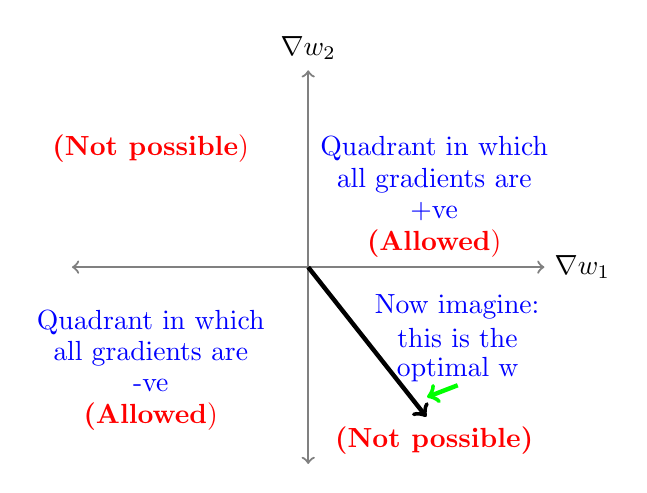
\begin{tikzpicture}

	\onslide<1-3>{
		\draw [thick, gray, <->] (10,2) -- (10,7)      % draw y-axis line
		node [above, black] {$\nabla w_2$};              % add label for y-axis
		%node [below,black]{$-y$};
		\draw [thick, gray, <->] (7,4.5) -- (13,4.5)      % draw x-axis line
		node [right, black] {$\nabla w_1$};              % add label for x-axis
	}


	\onslide<2-3>{\node[blue](text) at (8,6){\textcolor{red}{\textbf{(Not possible})}};}
	\onslide<2-3>{\node[blue](text) at (11.6,6){Quadrant in which};}
	\onslide<2-3>{\node[blue](text) at (11.6,5.6){all gradients are};}
	\onslide<2-3>{\node[blue](text) at (11.6,5.2){+ve};}
	\onslide<2-3>{\node[blue](text) at (11.6,4.8){\textcolor{red}{\textbf{(Allowed})}};}

	\onslide<2-3>{\node[blue](text) at (8,3.8){Quadrant in which};}
	\onslide<2-3>{\node[blue](text) at (8,3.4){all gradients are};}
	\onslide<2-3>{\node[blue](text) at (8,3){-ve};}
	\onslide<2-3>{\node[blue](text) at (8,2.6){\textcolor{red}{\textbf{(Allowed})}};}
	\onslide<2-3>{\node[blue](text) at (11.6,2.3){\textcolor{red}{\textbf{(Not possible)}}};}

	\onslide<3>{
		\draw[->,draw=black,ultra thick](10,4.5)--(11.5,2.6);
		\draw[->,draw=green,ultra thick](11.899,3.0)--(11.51,2.85);
	}
	\onslide<3>{
		\node(textmarked1) at (11.892,4){\textcolor{blue}{Now imagine:}};
		\node(textmarked2) at (11.896,3.6){\textcolor{blue}{this is the}};
		\node(textmarked3) at (11.899,3.2){\textcolor{blue}{optimal w}};

	}
	
\end{tikzpicture} 